\chapter{Domainmodell}

\section{Architekturmodell}
	Der logische Aufbau der Software besteht aus vier Schichten:
	\begin{figure}[h]
		\centering
		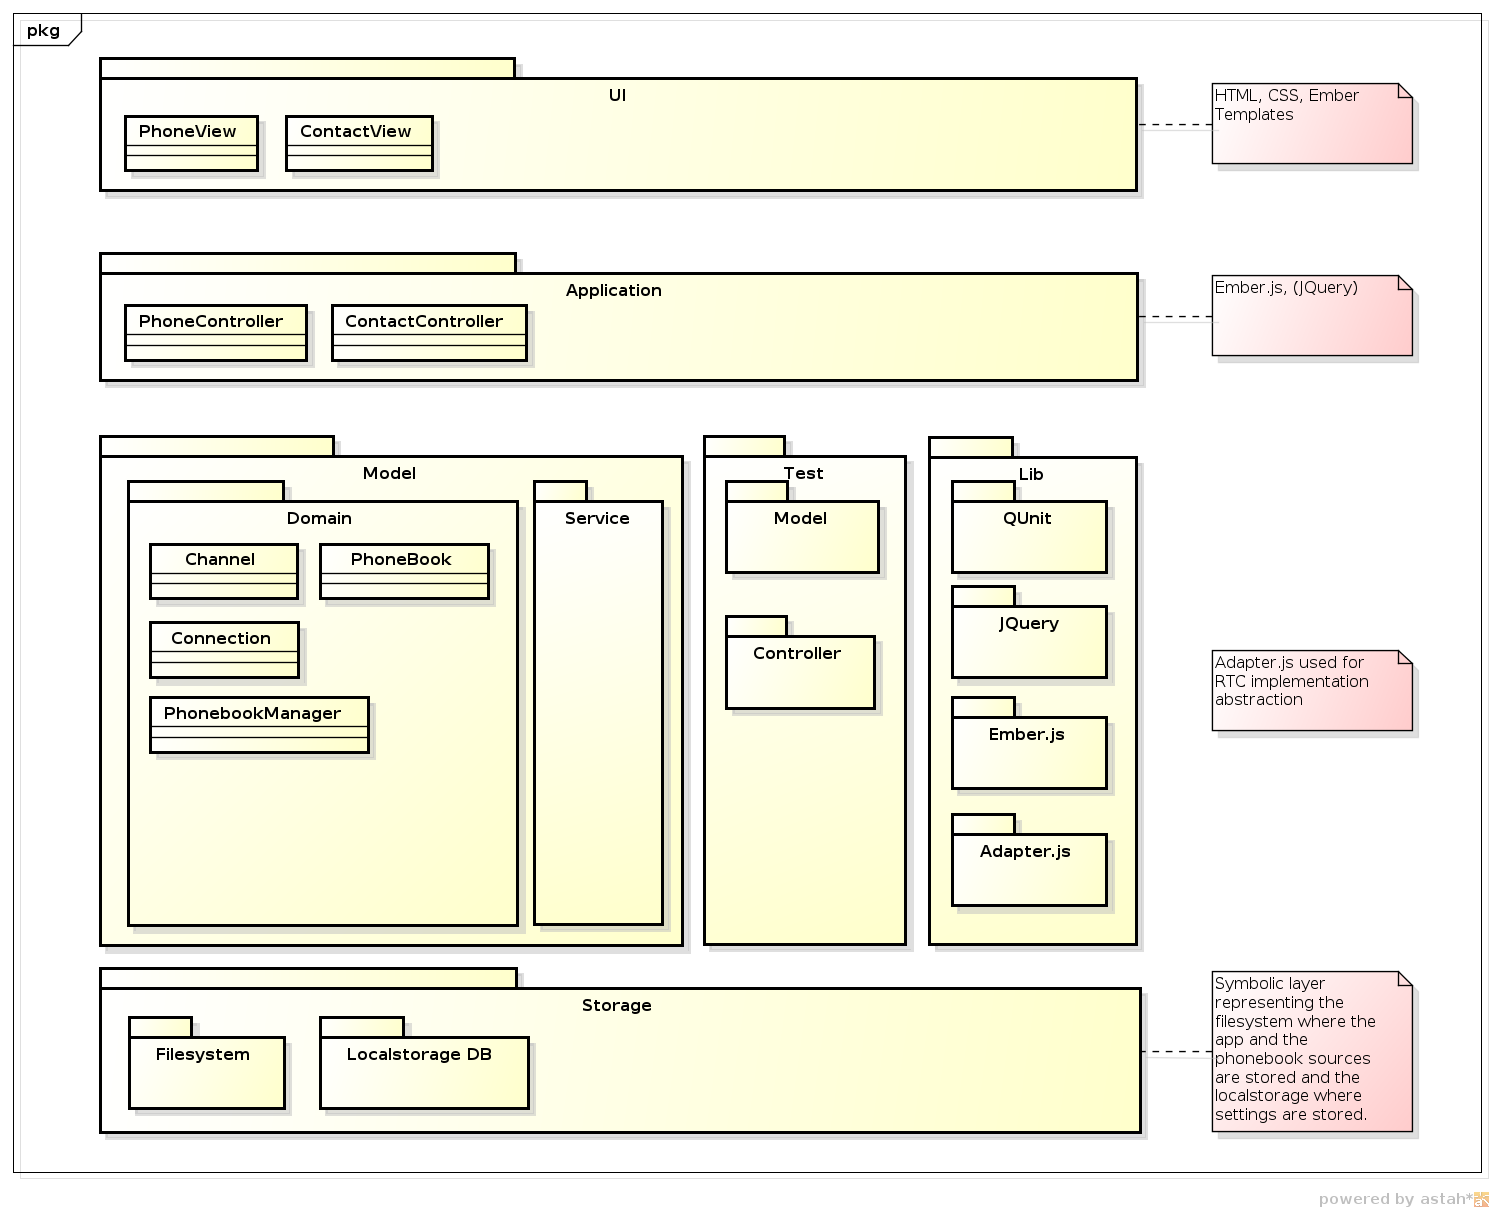
\includegraphics[width=1\textwidth]{img/architecture.png}
		\caption{Architekturdiagramm JS VoIP App}
	\end{figure}

	\begin{landscape}
		\section{Strukturdiagramm}
			Im folgenden Diagramm sind die wichtigsten konzeptionellen Klassen und ihre Beziehungen untereinander aufgeführt.
			\begin{figure}[h]
				\centering
				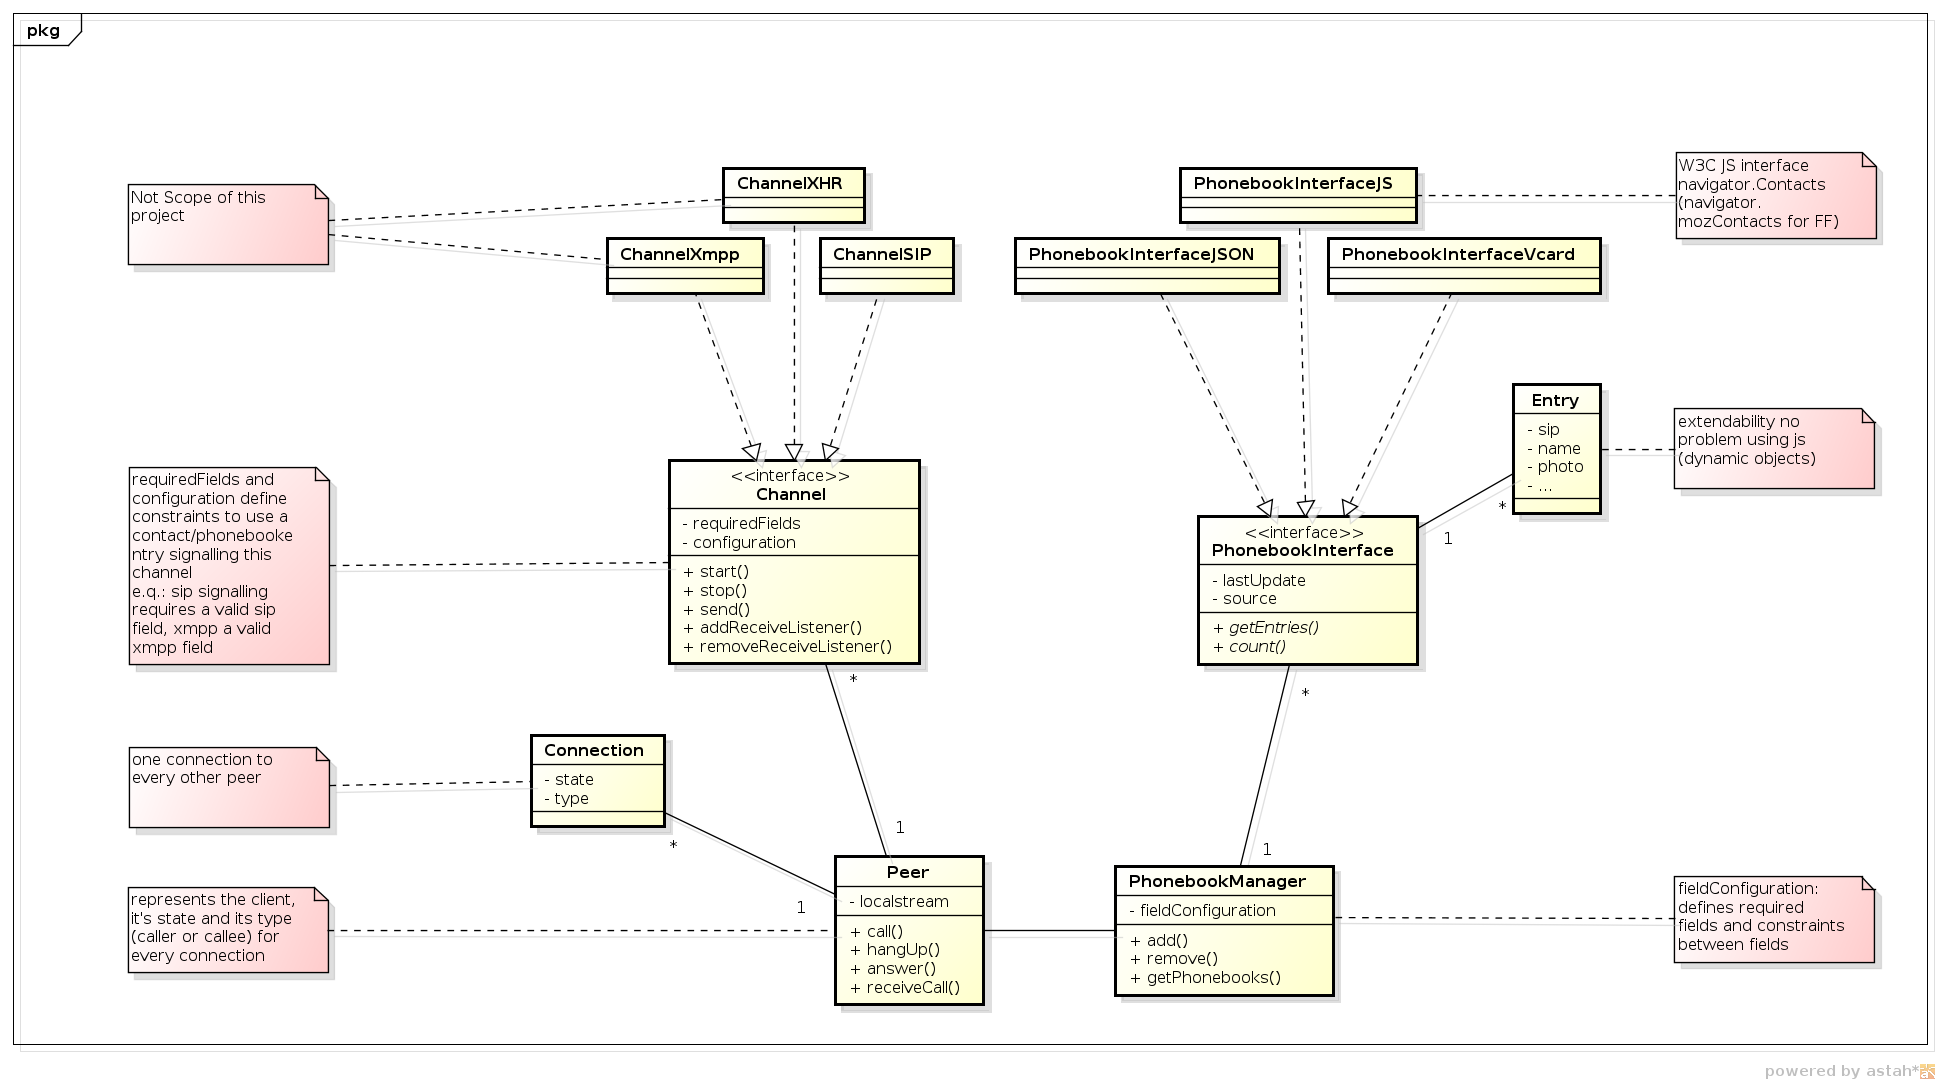
\includegraphics[width=1.2\textwidth]{img/domain.png}
				\caption{Strukturdiagramm JS VoIP App}
			\end{figure}
	\end{landscape}
	\clearpage

\section{Deployment}
	Die Applikation wird als ZIP-Datei ausgeliefert oder auf einem Webserver zur Verfügung gestellt. Der Benutzer kann die Datei entpacken und die darin enthaltene HTML Datei mit seinem Browser öffnen.
	\begin{figure}[h]
		\centering
		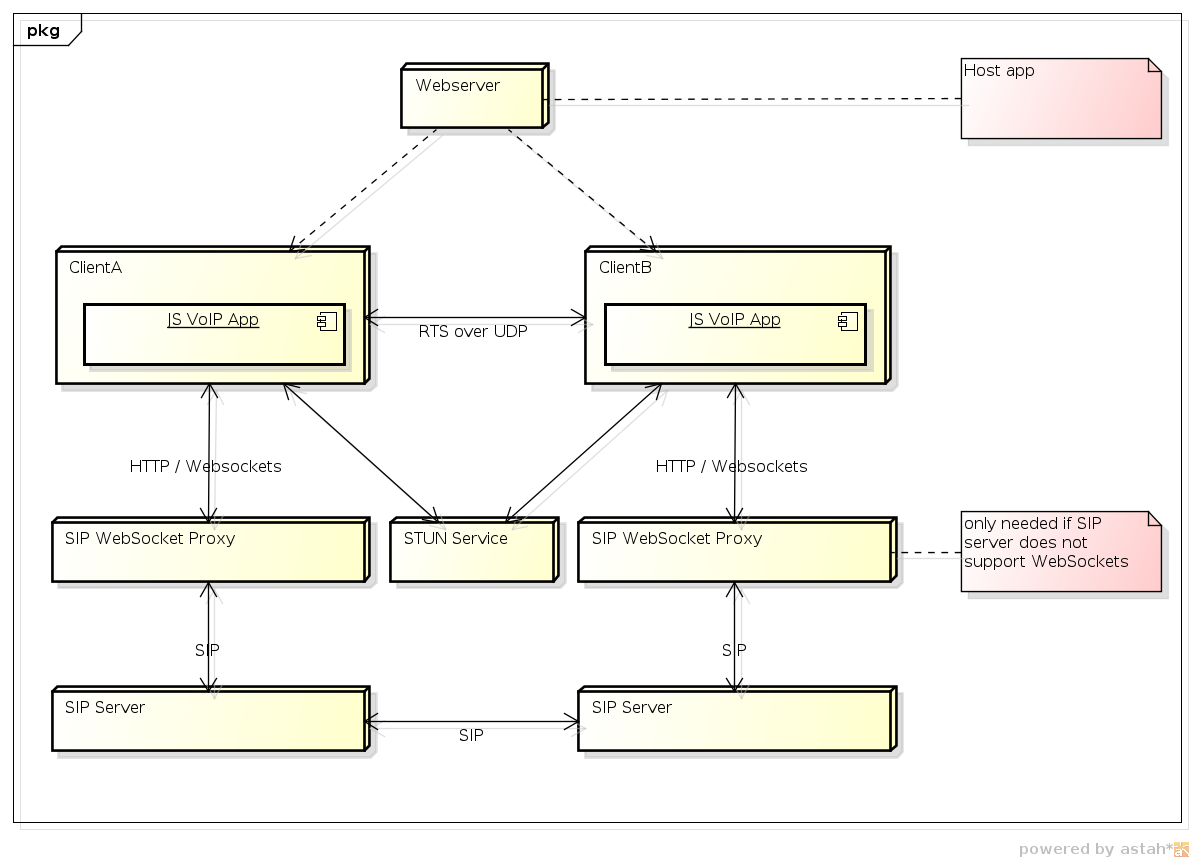
\includegraphics[width=1\textwidth]{img/deployment.png}
		\label{img:deployment}
		\caption{Deploymentdiagramm JS VoIP App}
	\end{figure}

\section{Architektur Designmotivations}
	\subsection{Client/Server vs. reine Client Applikation}
		\subsubsection{Vorteile Client-/Server Umsetzung}
		\begin{itemize}
			\item Schlanker Client
			\item Es wird nur eine Schnittstelle benötigt zwischen Client und Server, der gesammte Verkehr kann über HTTP abgewickelt werden.
			\item Nur der Server muss die Schnittstellen zu andern Diensten unterstützen. Keine zusätzlichen Schnittstellenanforderungen an den Client
		\end{itemize}
		\subsubsection{Nachteile}
		\begin{itemize}
			\item Redundanzen, da Funktionalität zwischen dem Client und Server durch ein eigene Protokoll erneut übersetzt wird und damit auf beiden Seiten Teile der gleichen Funktionalität umgesetzt werden müssen.
			\item Ein Anwender ist an den Server, bzw. diese Serverimplementation gebunden. Die Applikation läuft nicht ohne den Server.
			\item Server ist ``Single Point of Failure''
			\item Sollen weitere Schnittstellen umgesetzt werden, so muss der Server erweitert werden, was aufwendiger ist als den Client zu erweitern
		\end{itemize}


		\subsubsection{Vorteile reine Client Lösung}
		\begin{itemize}
			\item Es wird kein Server benötigt
			\item Anwender können einen beliebigen Kommunikationsserver (SIP) verwenden, bzw. sogar eine eigene Channelimplementation hinzufügen um z.B. über XMPP das Signalling durchzuführen
			\item Um die Applikation für weitere Schnittstellen zu erweitern sind keine Kenntnisse der Servertechnologie notwendig
			\item Die Applikation insgesammt ist weniger aufwändig aufgebaut weil sie weniger Redundanzen beinhaltet
		\end{itemize}
		\subsubsection{Nachteile}
		\begin{itemize}
			\item Die möglichen Schnittstellen sind auf Browserfunktionalität begrenzt (HTTP, WebSockets, RTSP). Dadurch muss ein SIP oder XMPP Provider WebSockets unterstützen, damit er für das Signalling benutzt werden kann.
			\item Der Client wird etwas umfangreicher
		\end{itemize}

		\subsubsection{Fazit}
			Aufgrund geringerer Abhängigkeiten und der Wahrscheinlichkeit, das SIP Server Provider irgendwann WebSockets unterstützen, wird die Lösung ``reine Client Applikation'' gewählt.
			Für die Kommunikation mit Signallingservern wie SIP oder XMPP werden WebSockets eingesetzt, für Signalling über XHR wird mit der Option ``Allow Cross Origin'' gearbeitet.

	\subsection{STUN Service}
		STUN Services sind zwingend notwendig um die nach aussen sichtbare IP Adresse des Clients herauszufinden. Nebst der Möglichkeit selbst einen STUN Service aufzusetzen, gibt es frei verfügbare STUN Services, z.B. von Mozilla oder Google.


		Für ein Abgeschottetes Netz ist ein eigener STUN Server zwingend notwendig. Für unsern Fall reichen die frei verfügbaren. Durch anpassen der Konfiguration ist es möglich den Server festzulegen.


	\subsection{SIP Proxy vs. SIP Server mit WebSockets}
		Unterstützt ein SIP Server keine WebSockets, so kann ein SIP/WebSocket Proxy dazwischen geschaltet werden. Die Konfiguration eines SIP Proxies ist ähnlich aufwändig wie die Installation eines Kamailio SIP Servers, der in der neusten Version WebSockets unterstützt.


		Aus diesem Grund wird ein eigener SIP Server dem Proxy vorgezogen.


	\subsection{Hosting}
		Die JS VoIP App kann sowohl lokal ausgeführt werden wie von einem Webserver ausgeliefert ausgeführt werden. Es gibt keine speziellen Voraussetzungen. Ein Webserver ist daher nicht zwingend notwendig.
	
